


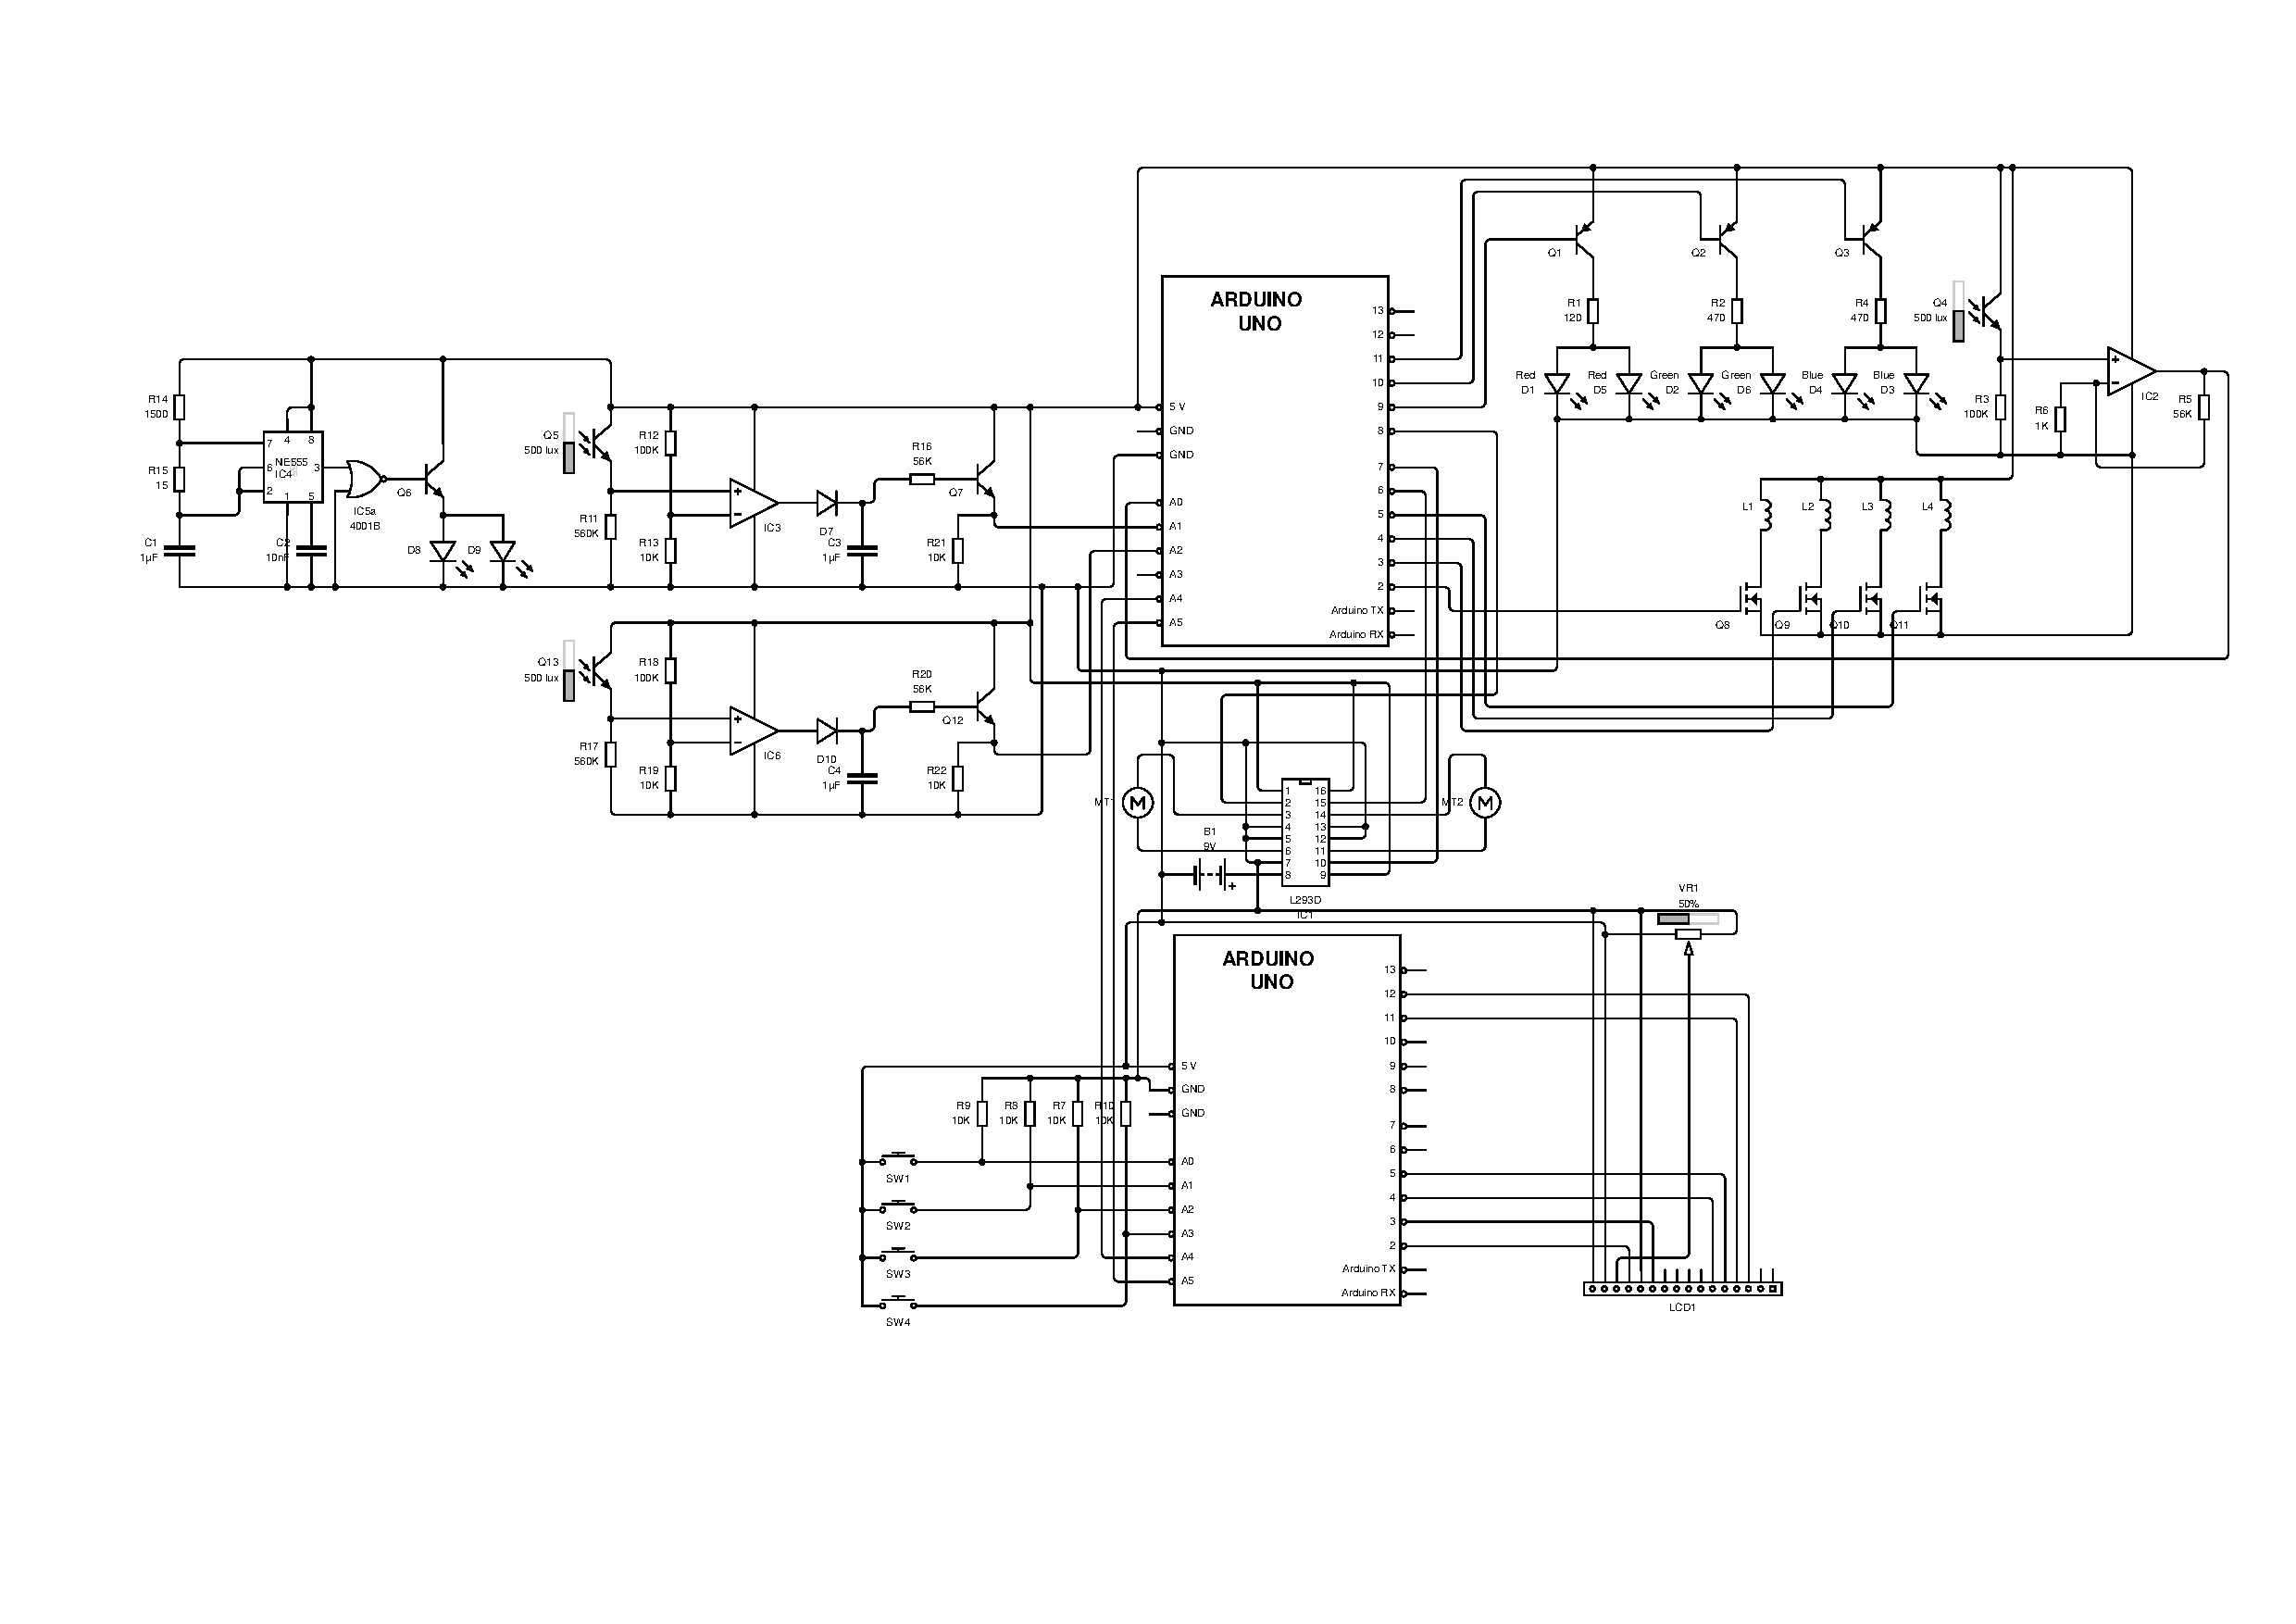
\includepdf[pages=1,fitpaper,pagecommand={\section{Samlet kredsløb} \label{bilag:samletkreds}}]{figures/CIRCUITS/samletFINAL}

% pagecommand={\section{Samlet kredsløb} \label{bilag:samletkreds}}


\section{Endelig prototype - kredsløb} \label{bilag:endeligprotokreds}
\begin{center}
	\includegraphics[width=15cm]{figures/2_5fremstilling/prototyper/Endeligproto.png}
\end{center}

\section{Endelig prototype - kanonkonstruktion} \label{bilag:endeligprotokanon}
\begin{center}
	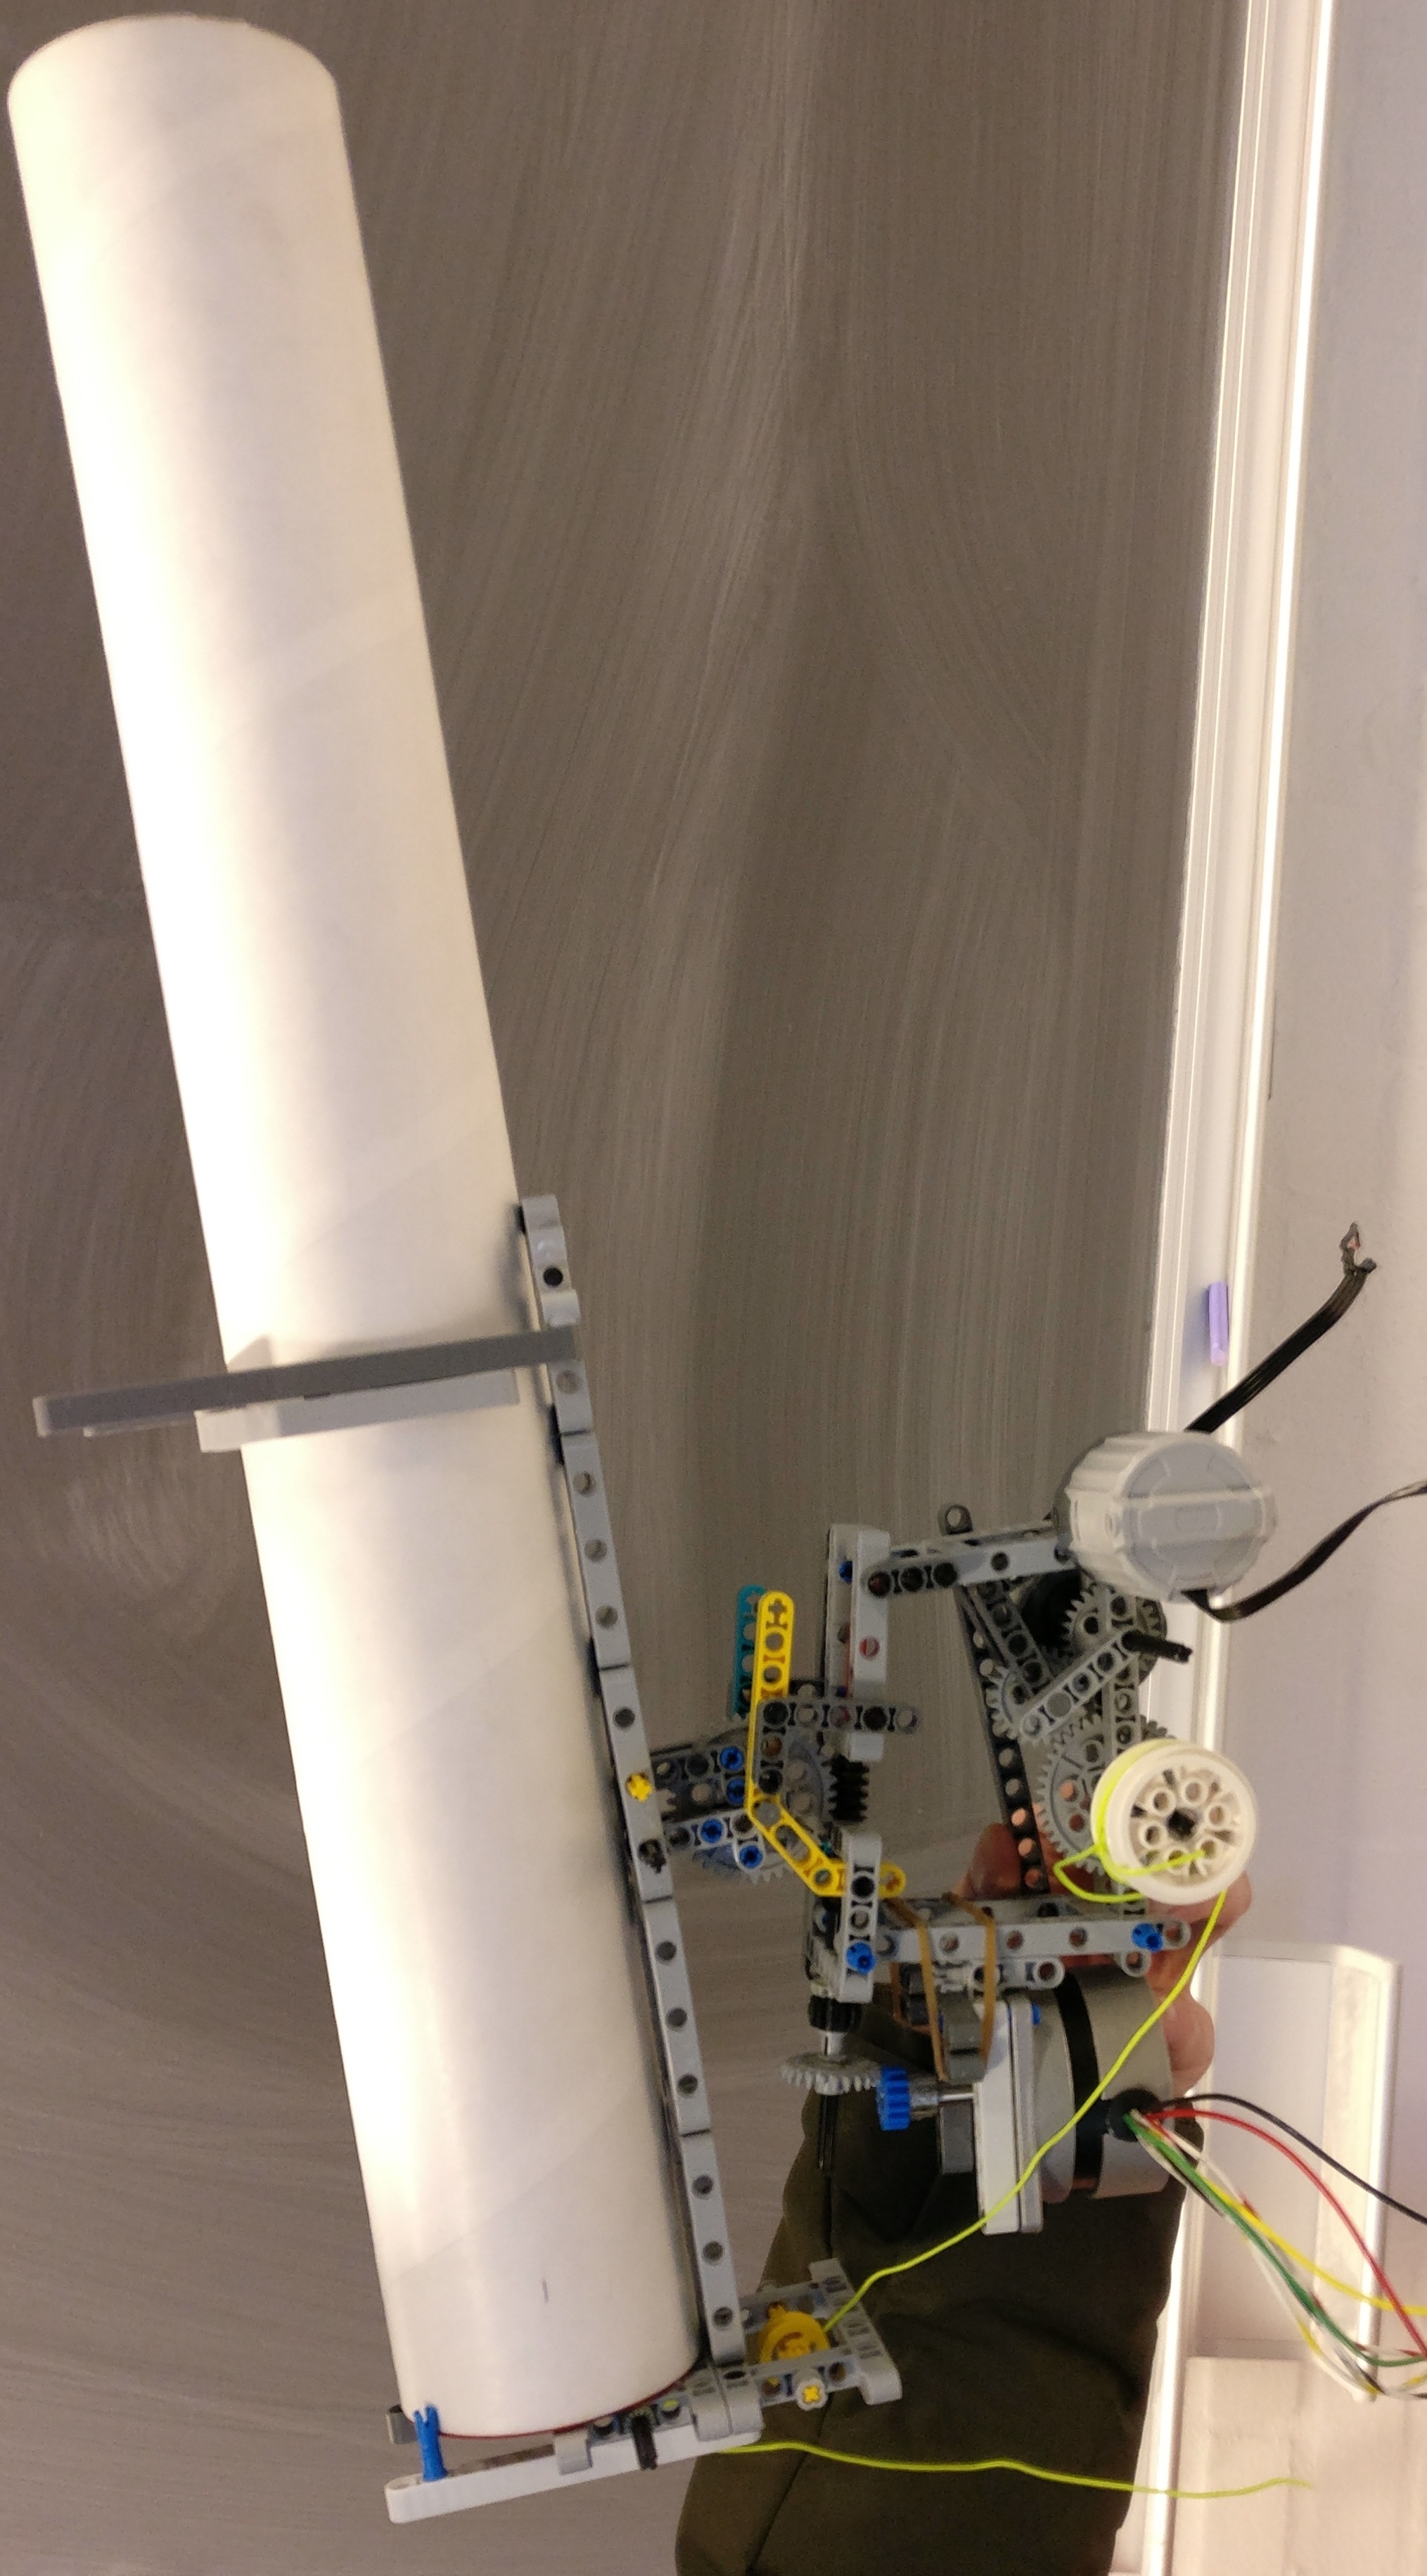
\includegraphics[height=20cm]{figures/2_5fremstilling/prototyper/paenkanon.jpg}
\end{center}
\section{PCB artwork til hastighedssensor}\label{bilag:afsenderModtagerArtwork}
\begin{figure}[H]
	\centering
    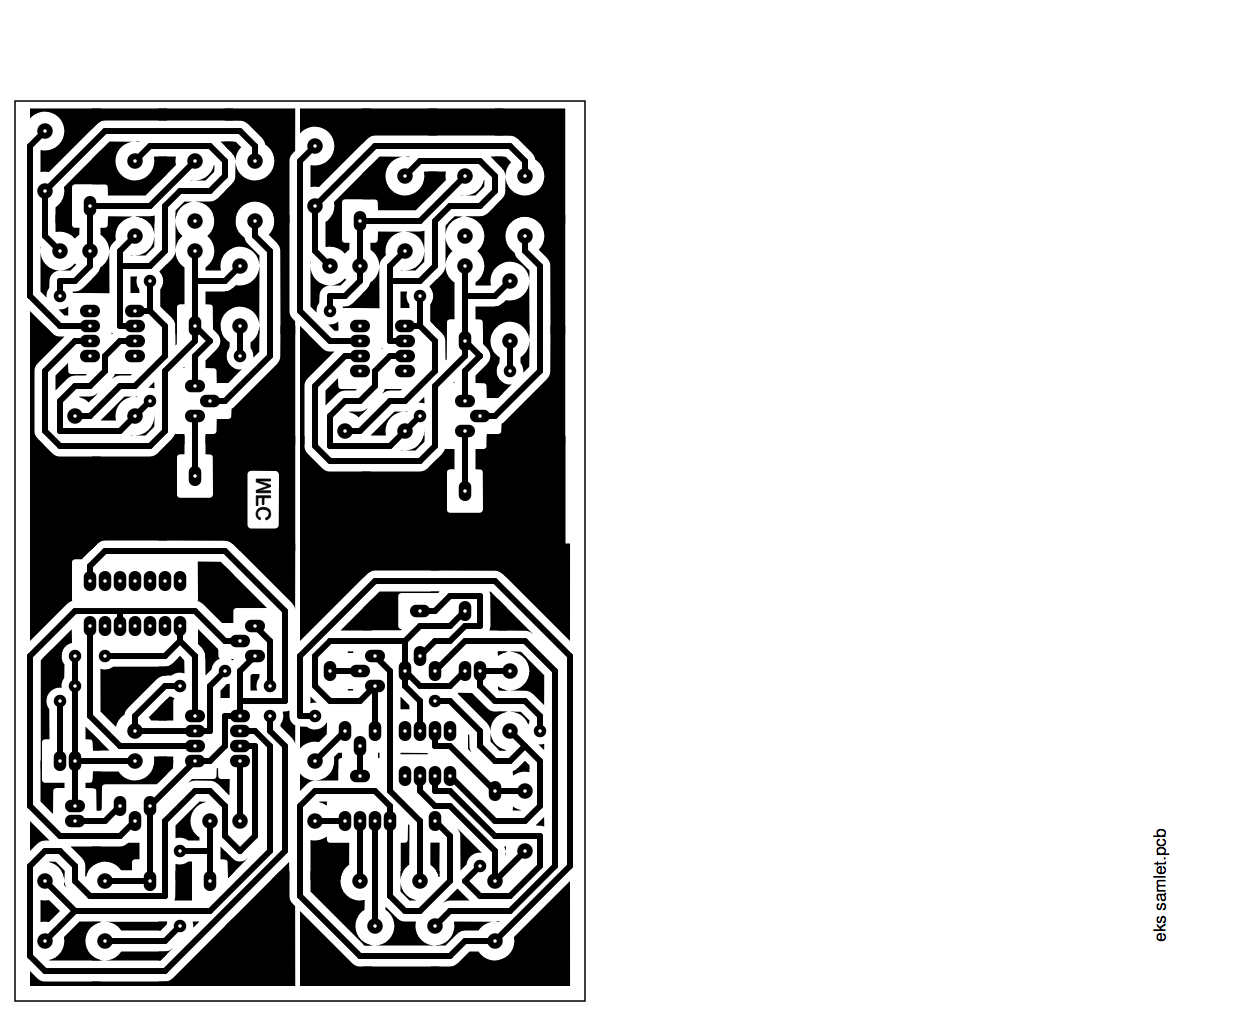
\includegraphics[width=210mm]{figures/2_5fremstilling/afsenderModtagerArtwork.png}
\end{figure}


\section{PCB artwork til arduino shield} \label{bilag:shieldArtwork}
\begin{figure}[H]
	\centering
    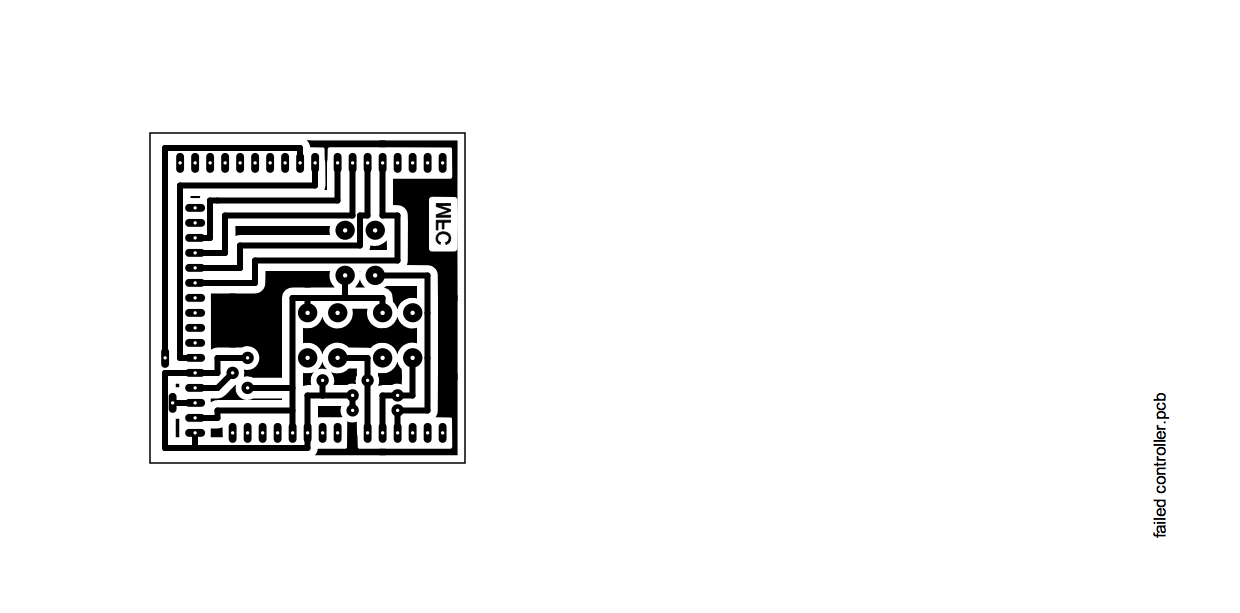
\includegraphics[width=210mm]{figures/2_5fremstilling/shieldArtwork.png}
\end{figure}

\todo{Måske skulle vi overveje at lave et nyt billede med samlede kabler}
\begin{figure}[H]
\section{Fumlebrætmodel anden del}
	\centering
    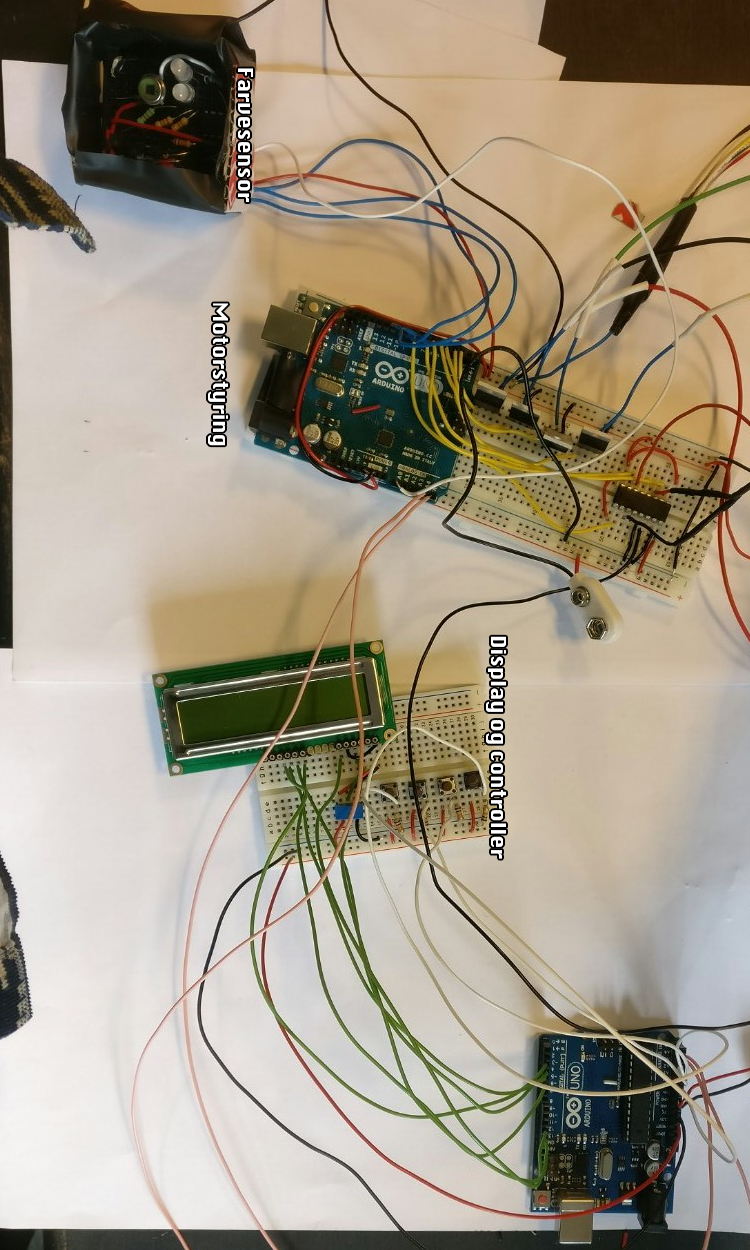
\includegraphics[width=13cm]{figures/2_5fremstilling/prototyper/rumleKreds.png}
\end{figure}


% Must be second last (the longer the later)
\section{Program til Master Arduino}
\label{bilag:programMaster}
\begin{lstlisting}

\end{lstlisting}

\section{Program til Controller Arduino}
\label{bilag:programController}
\begin{lstlisting}

\end{lstlisting}

% MUST BE LAST
\section{Logbog} 